
%In the following, we first present the performance comparison between original registry and \sysname.
%Next, we present the layer restoring performance.

\subsection{Deduplication Performance}
\label{sec:eval-dedup}

%We map the traces with two different layer groups: 
%small layers (layer size $\leq$ 50 MB)

\begin{figure*}[t]
	\centering
	\begin{minipage}{0.3\textwidth}
		\centering
		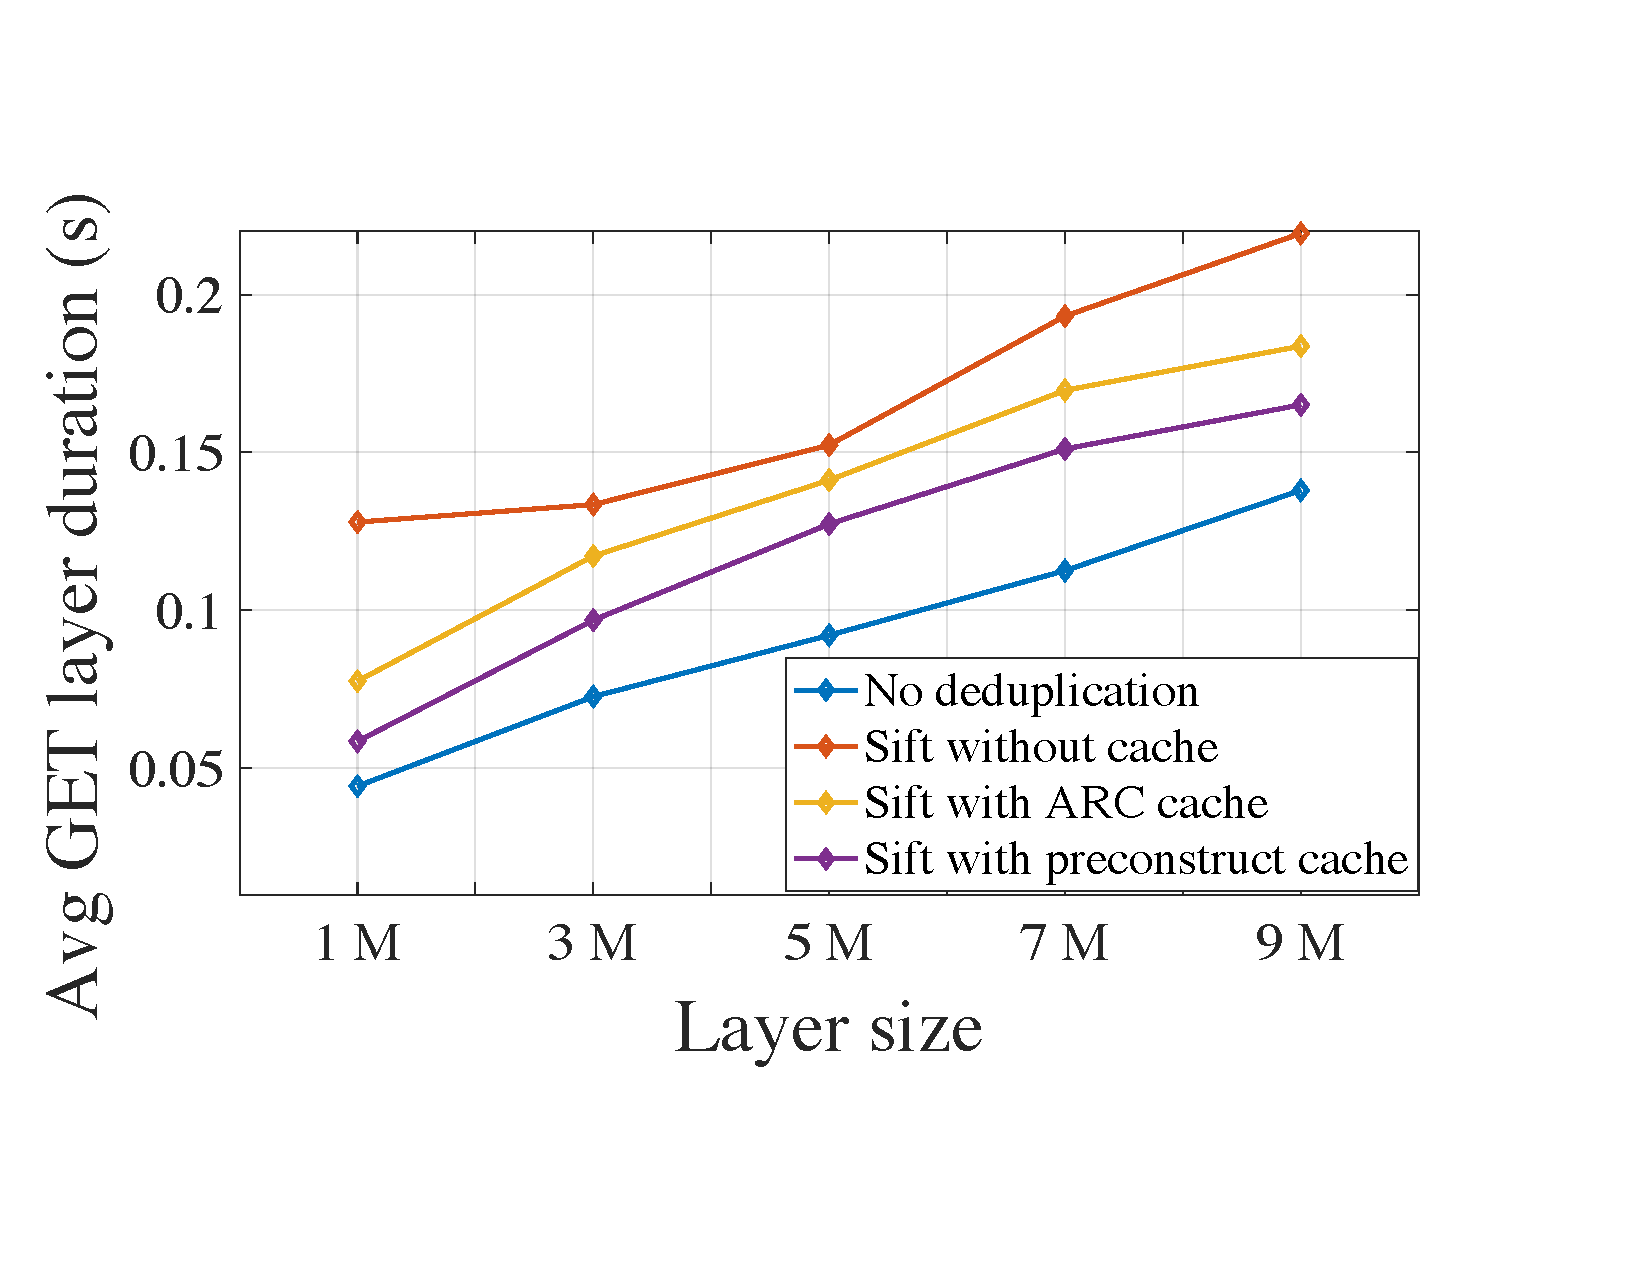
\includegraphics[width=\textwidth]{graphs/1nodegetlayerlatency.pdf}
		\caption{GET layer latency}
		\label{fig:eval-1nodegetlayerlatency}
	\end{minipage}%
\hspace{1mm}
	\begin{minipage}{0.29\textwidth}
		\centering
		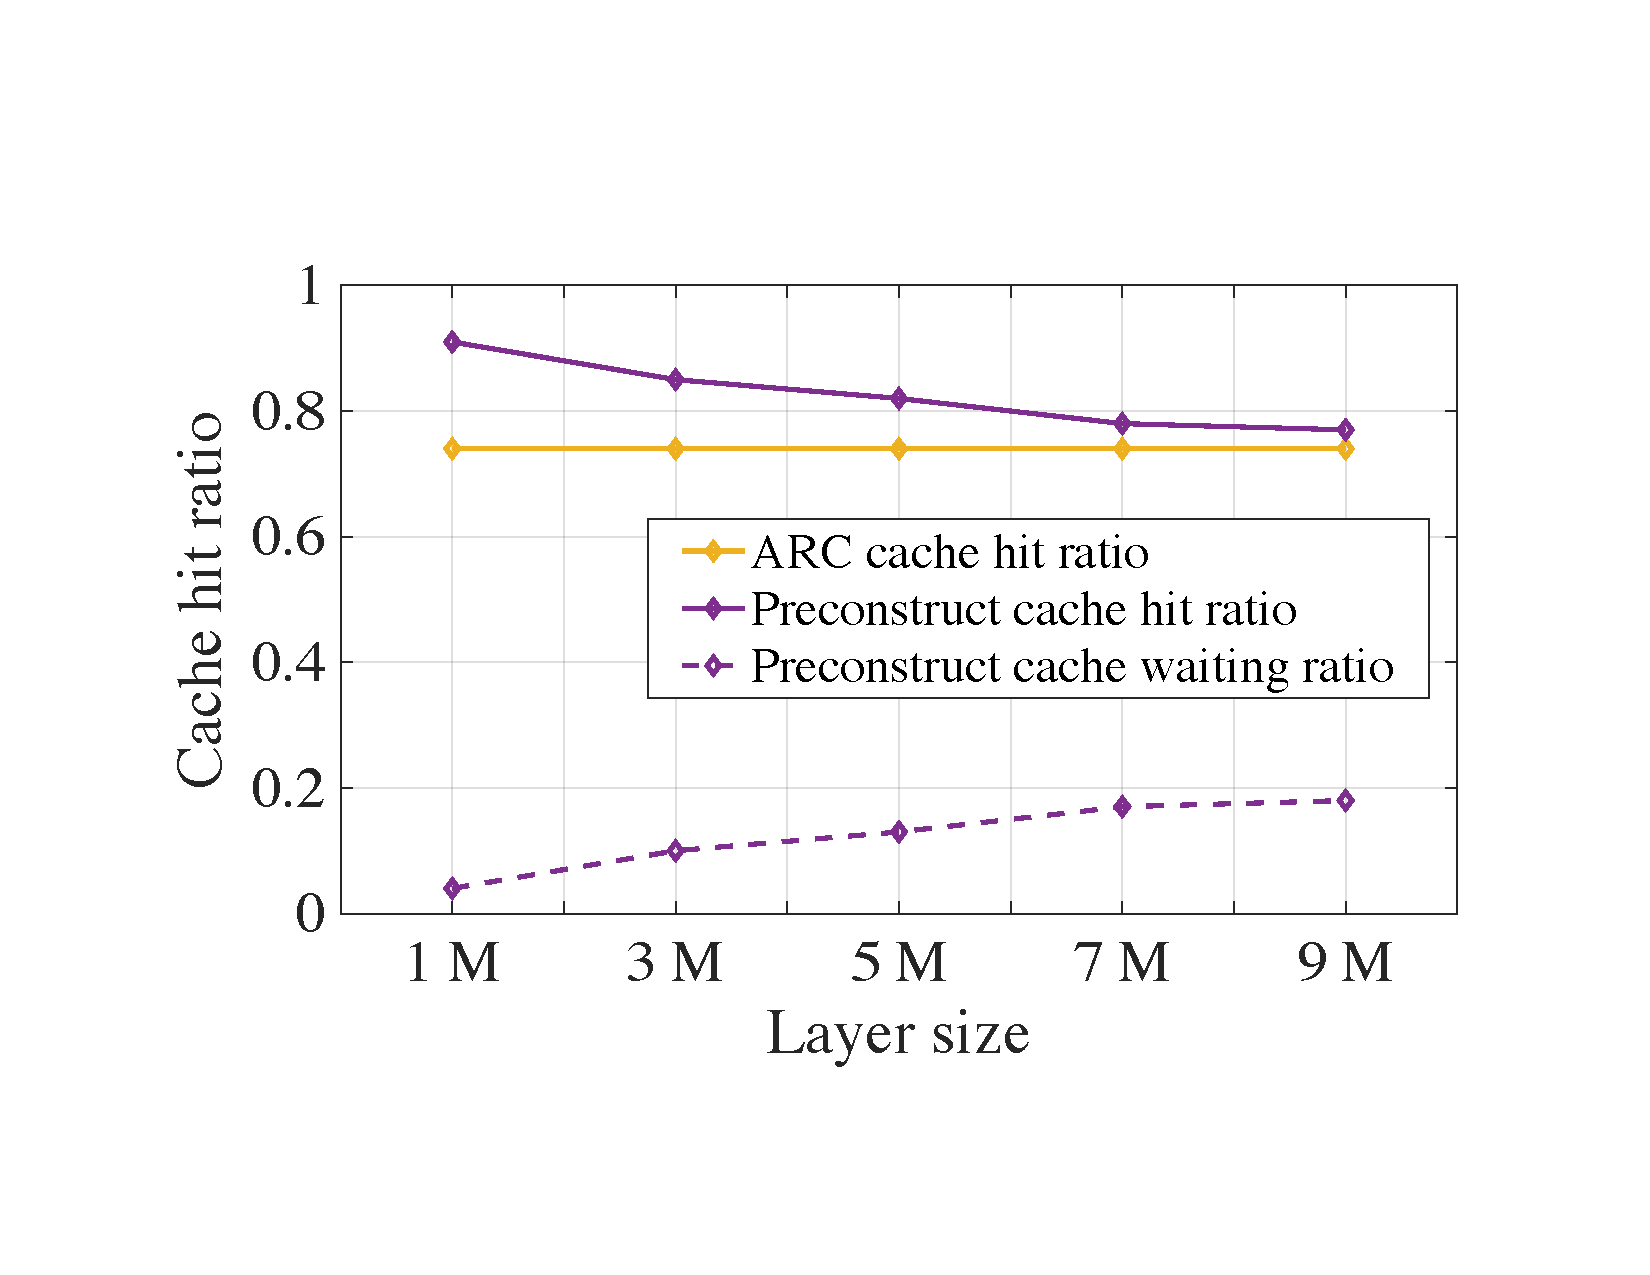
\includegraphics[width=\textwidth]{graphs/cachehitratio.pdf}
		\caption{Cache hit ratio}% of LRU cache and preconstruct cache.}
		\label{fig:eval-cachehitratios}
	\end{minipage}%
\hspace{1mm}
	\begin{minipage}{0.28\textwidth}
	\centering
	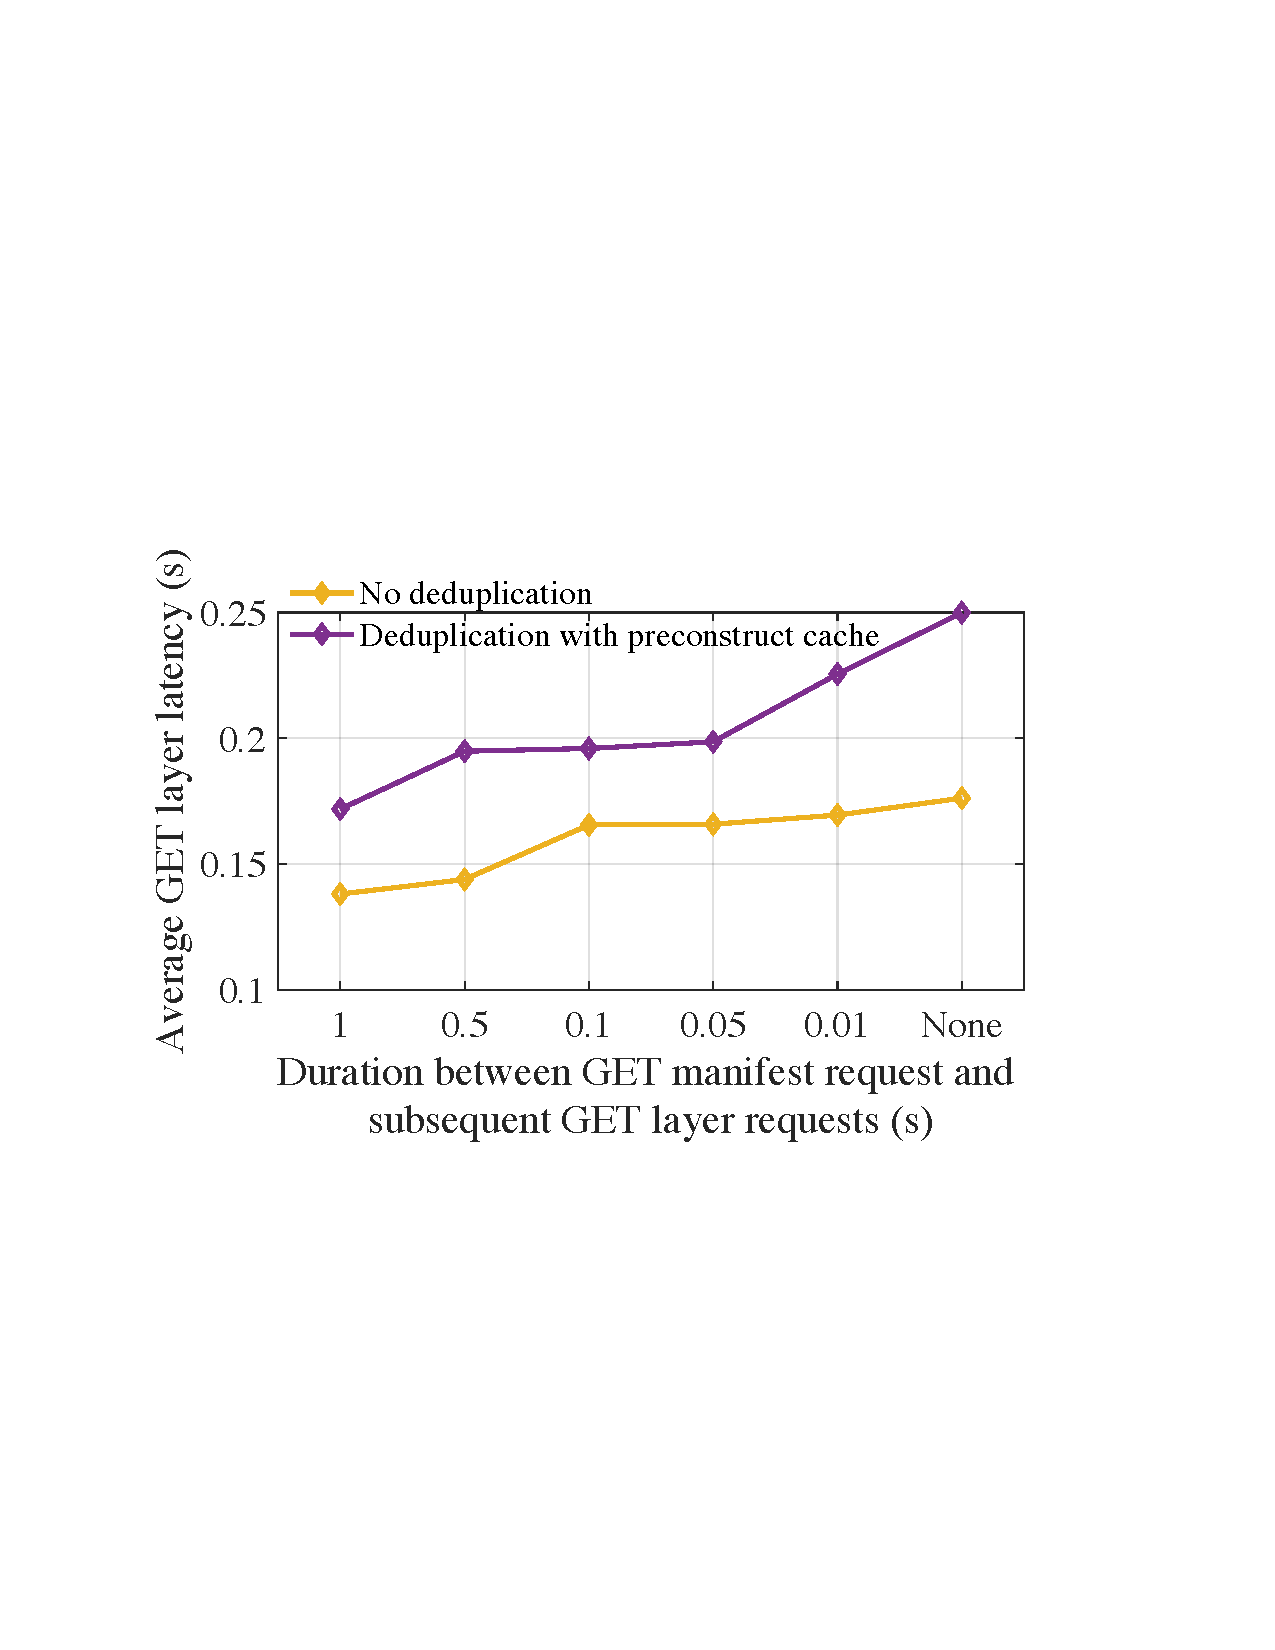
\includegraphics[width=\textwidth]{graphs/durationML.pdf}
	\caption{\texttt{GET} manifest/layer IAT}
	\label{fig:eval-durationML}
   \end{minipage}
\end{figure*}

In this section, we evaluate the layer restoring latency of \sysname's deduplication cluster 
and its impact on \texttt{GET} layer request latency.
%
We first measure a single D-server's layer restoring capability and compare it with 
a \emph{no deduplication} scheme, i.e.  a plain registry server with a local file system backend
that performs no deduplication.
%
Then we scale out to a deduplication cluster with multiple D-servers and compare
\sysname to BOLT~\cite{littley2019bolt}, a recently published, state-of-the-art registry design.
%
%a consistent hashing based distributed docker registry cluster 
%that utilizes the local file systems on the nodes for storage.
%
%
% (denoted as
%\sysname-dedup)
% and 
%overhead of layer deduplication on .
%To measure the  
%We compare the \texttt{GET} layer latency of D-servers
%with 
%by running \sysname with \text{only deduplication} on a single D-server.
%We launch a client on another server and \texttt{pulls} 3 layers in parallel.
%We configure \sysname as
%registry without deduplication,
%deduplication registry,
%deduplication registry with LRU cache~\cite{xxx},
%and
%deduplication registry with a preconstruct cache.
%We set the cache size as 20\% of ingress data.

\paragraph{Restoring latency}
%
%\LR{Why are we only looking at layers between 1 and 9\,MB?}
%\NZ{We start from small layers to big layers like 70 MB.
%small layers can be restored by using just a single node.}
%\LR{Is the ARC cache the layer stage area cache or what does it refer to in Figure 3a?}
%\NZ{No. ARC cache is a layer cache which stores the constructed hot layers
%to save restoring time. ARC cache does not preconstruct layers.}
%
To evaluate \sysname{}'s restoring latency, we launch a single node registry on a server
and use one client on a separate machine.
%
We compare four different configurations:
(1)~no deduplication;
(2)~\sysname without caching;
(3)~\sysname with ARC caching but no preconstruction; and
(4)~\sysname with preconstruct cache.
%
For each setup, we use the local file system as the storage backend and replay the
\dal workload with layer size groups from 1\,MB to 9\,MB. For this experiment, we focus
only on smaller layers as our registry setup is single-node.
%
%\LR{Above we say we match layers randomly?}
%\NZ{yes}
%
%The client matches requests from \dal to layers with similar sizes 
%from the evaluation dataset and replays them to the D-server.
%We compare four backends: 

%\LR{Do we also have percentiles/errorbars or just averages?}
%\NZ{we have 90th percentile.}
%
As shown in Figure~\ref{fig:eval-1nodegetlayerlatency}, 
layer restoring increases the average \texttt{GET} layer request latency by 189\% for layers 
with size 1\,MB for \sysname without caching compared to \emph{no deduplication}.
%
Moreover, the layer restoring latency increases almost linearly as the layer size increases.
%
While a 1\,MB layer takes 0.13\,s to restore and download, 
it takes 0.22\,s for a 9\,MB layer for \sysname without caching.

%\paragraph{Preconstruct cache VS. ARC cache}
%\paragraph{Cache}
%
The results show that
%As shown in Figure~\ref{fig:eval-1nodegetlayerlatency}, 
%the average \texttt{GET} layer request latency increase with the layer size.
leveraging a cache can largely reduce layer restoring latency.
%
When using an ARC cache, the layer restoring overhead decreases by 40\% for layers with
a size of 1\,MB compared to \sysname without cache.
%
However, as the layer size increases,  the improvement drops.
%
For 9\,MB layers, the presence of the ARC cache reduces the average layer restoring overhead by only 16\%
from the overhead of using Sift without caching.
%
%\LR{Do we have a reason for that?}
%\NZ{This is because it takes longer to restore a bigger layer upon a cache miss.}
%
%\Subil{there is no 10-MB value in Fig~\ref{fig:eval-1nodegetlayerlatency}.}
%ARC cache can only improve 10\% of 
%Restoring a layer puts 150\% overhead on \texttt{GET} layer latency.
%By adding a ARC cache,
%he average \texttt{GET} layer latency decreases by 39\%.
With the preconstruct cache, \sysname is able to improve \texttt{GET} layer latencies even further.
%
For 1\,MB layers, the average latency decreases by an additional 24\% compared to the ARC cache.
%
Overall, \sysname with preconstruct incurs the lowest overhead and only increases latencies by
19\% for layers with a 9\,MB size. 

\paragraph{Cache hit ratio}
%
Figure~\ref{fig:eval-cachehitratios} shows the cache hit ratios for the ARC and
preconstruct caches.
%
Note that the cache size is set to 20\% of \dal{}'s ingress data ,i.e. 20\% of the total size of
all unique layers, which are pushed to the registry as part of our workload.
%
%\NZ{Here, the cache size = unique layer count x layer size x 0.2.
%Cache size depends on the layer size we chose.
%we replay the workload five times, varying
%the layer size (from 1~MB to 9~MB)
%For example, if layer size is 1 M,
%then the cache size = unique layer count x I MB x 0.2
%= 1278*0.2MB.}
%
%\Subil{approximately how much is Dal's ingress data?}.
%
The cache hit ratio for ARC is stable at 0.77 for all layer sizes while
the preconstruct cache achieves a hit ratio of 0.95 for 1\,MB.

As the layer size increases to 9\,MB, the preconstruct cache hit ratio decreases to 79\%.
%
This is because the layer restoring latency increases with layer size as shown in
Figure~\ref{fig:eval-1nodegetlayerlatency} and therefore, some layers can not be preconstructed
on time.
%
%\LR{We should introduce waiting ratio here.}
%\NZ{The waiting ratio is calculated by the number of \texttt{GET} layer requests that are waiting for
%layer preconstruction process to finish divided by the total number of \texttt{GET} layer requests.}
%
This is indicated by the increasing number of waiting \texttt{GET} layer requests for larger layer
sizes, depicted by the preconstruct cache waiting ratio in Figure~\ref{fig:eval-cachehitratios}.
%
The waiting ratio is the number of \texttt{GET} requests that were blocked on reconstruction
divided by the total number of \texttt{GET} requests.
%
%Since layer construction already starts before these requests arrive, the restoring overhead can
%be reduced.
%
%\LR{The below is confusing, why is it the sum of the two?}
%\NZ{Its because prediction accuracy is calculated by the number of correct predictions divided by 
%total \texttt{GET} layer requests.
%The \texttt{GET} layer requests that are waiting for preconstruction to finish are also correct predictions.}
%
The user-behavior based request prediction accuracy is calculated by summing the preconstruct
cache hit ratio and the waiting ratio, i.e. all requests that successfully retrieved layers from the cache,
which results to 0.95.
%
%As shown in Figure~\ref{fig:eval-cachehitratios}, the prediction accuracy is 0.95.

\begin{figure*}[t]
	\centering
	\begin{minipage}{0.3\textwidth}
		\centering
		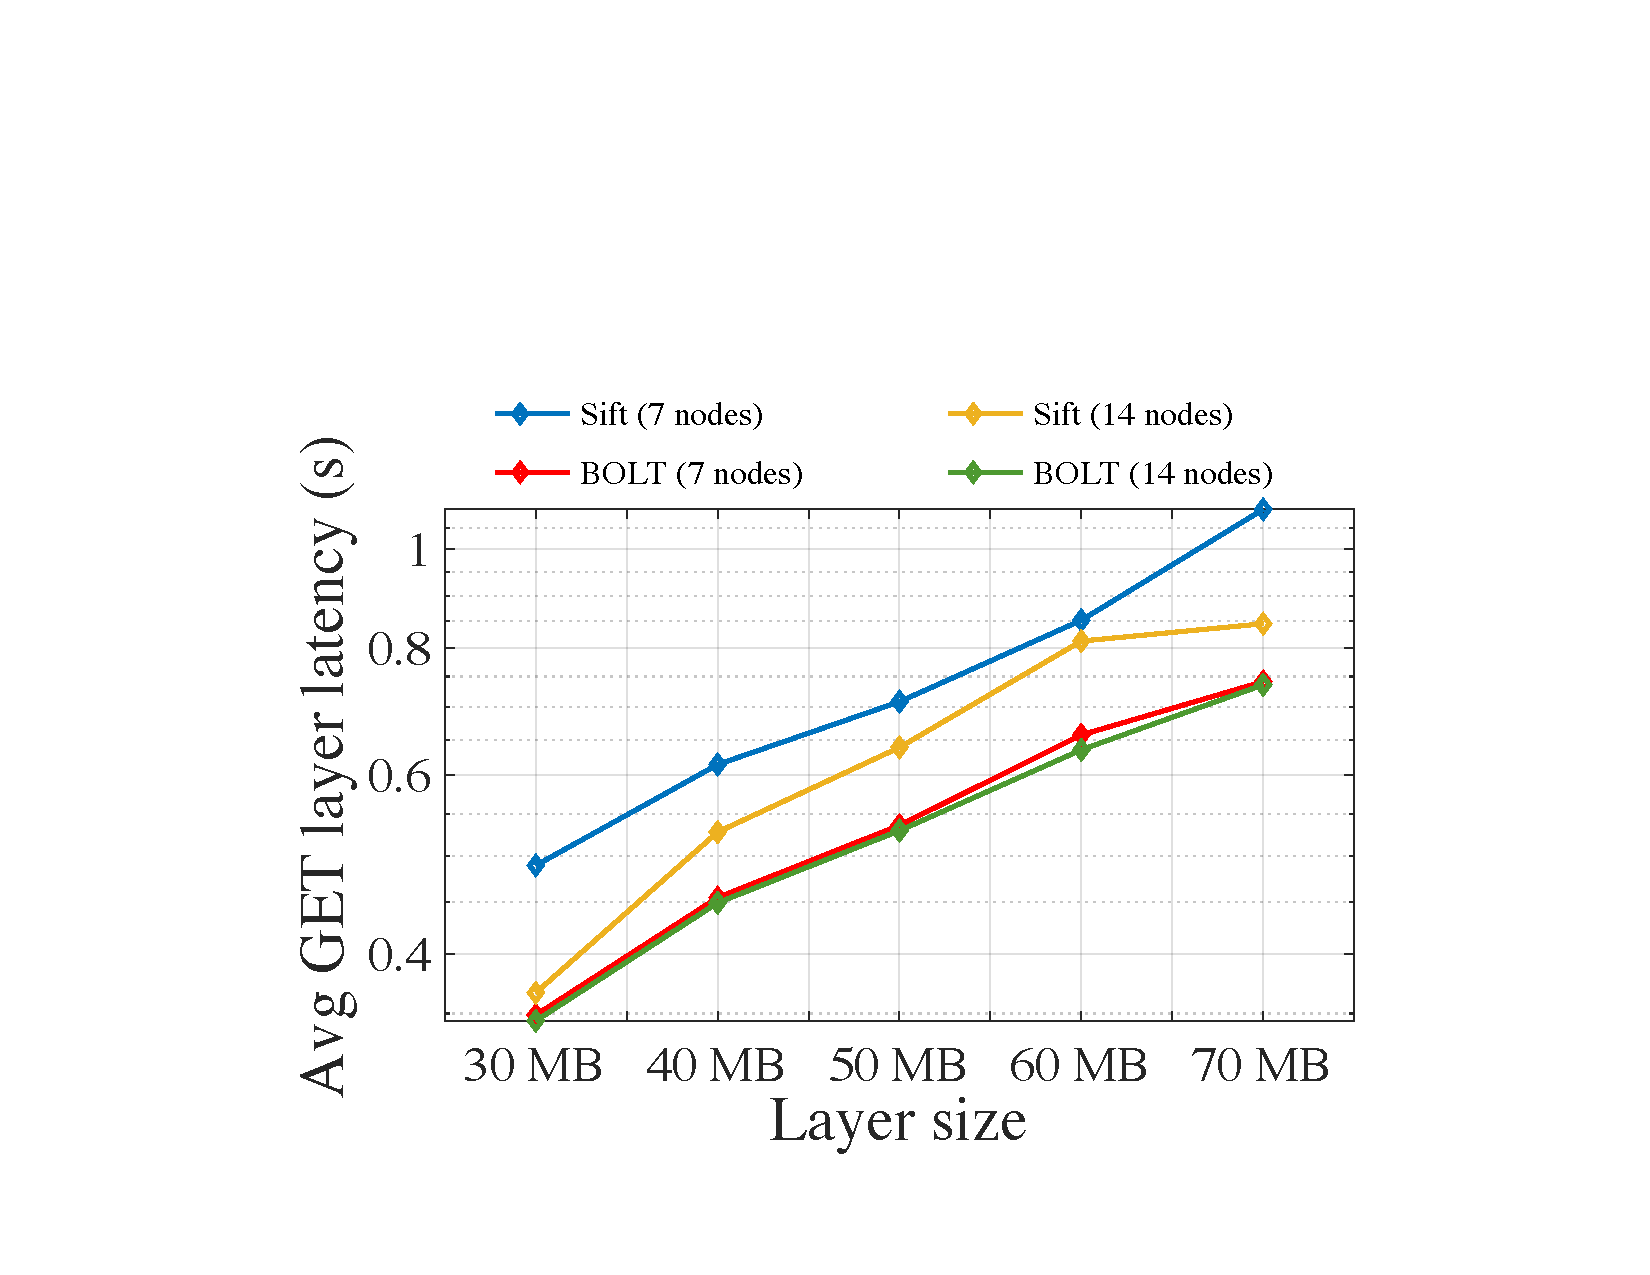
\includegraphics[width=\textwidth]{graphs/clusterscale.pdf}
		\caption{GET layer latency with different cluster size}
		\label{fig:eval-clusterscale}
	\end{minipage}%
	\hspace{1mm}
		\begin{minipage}{0.3\textwidth}
		\centering
		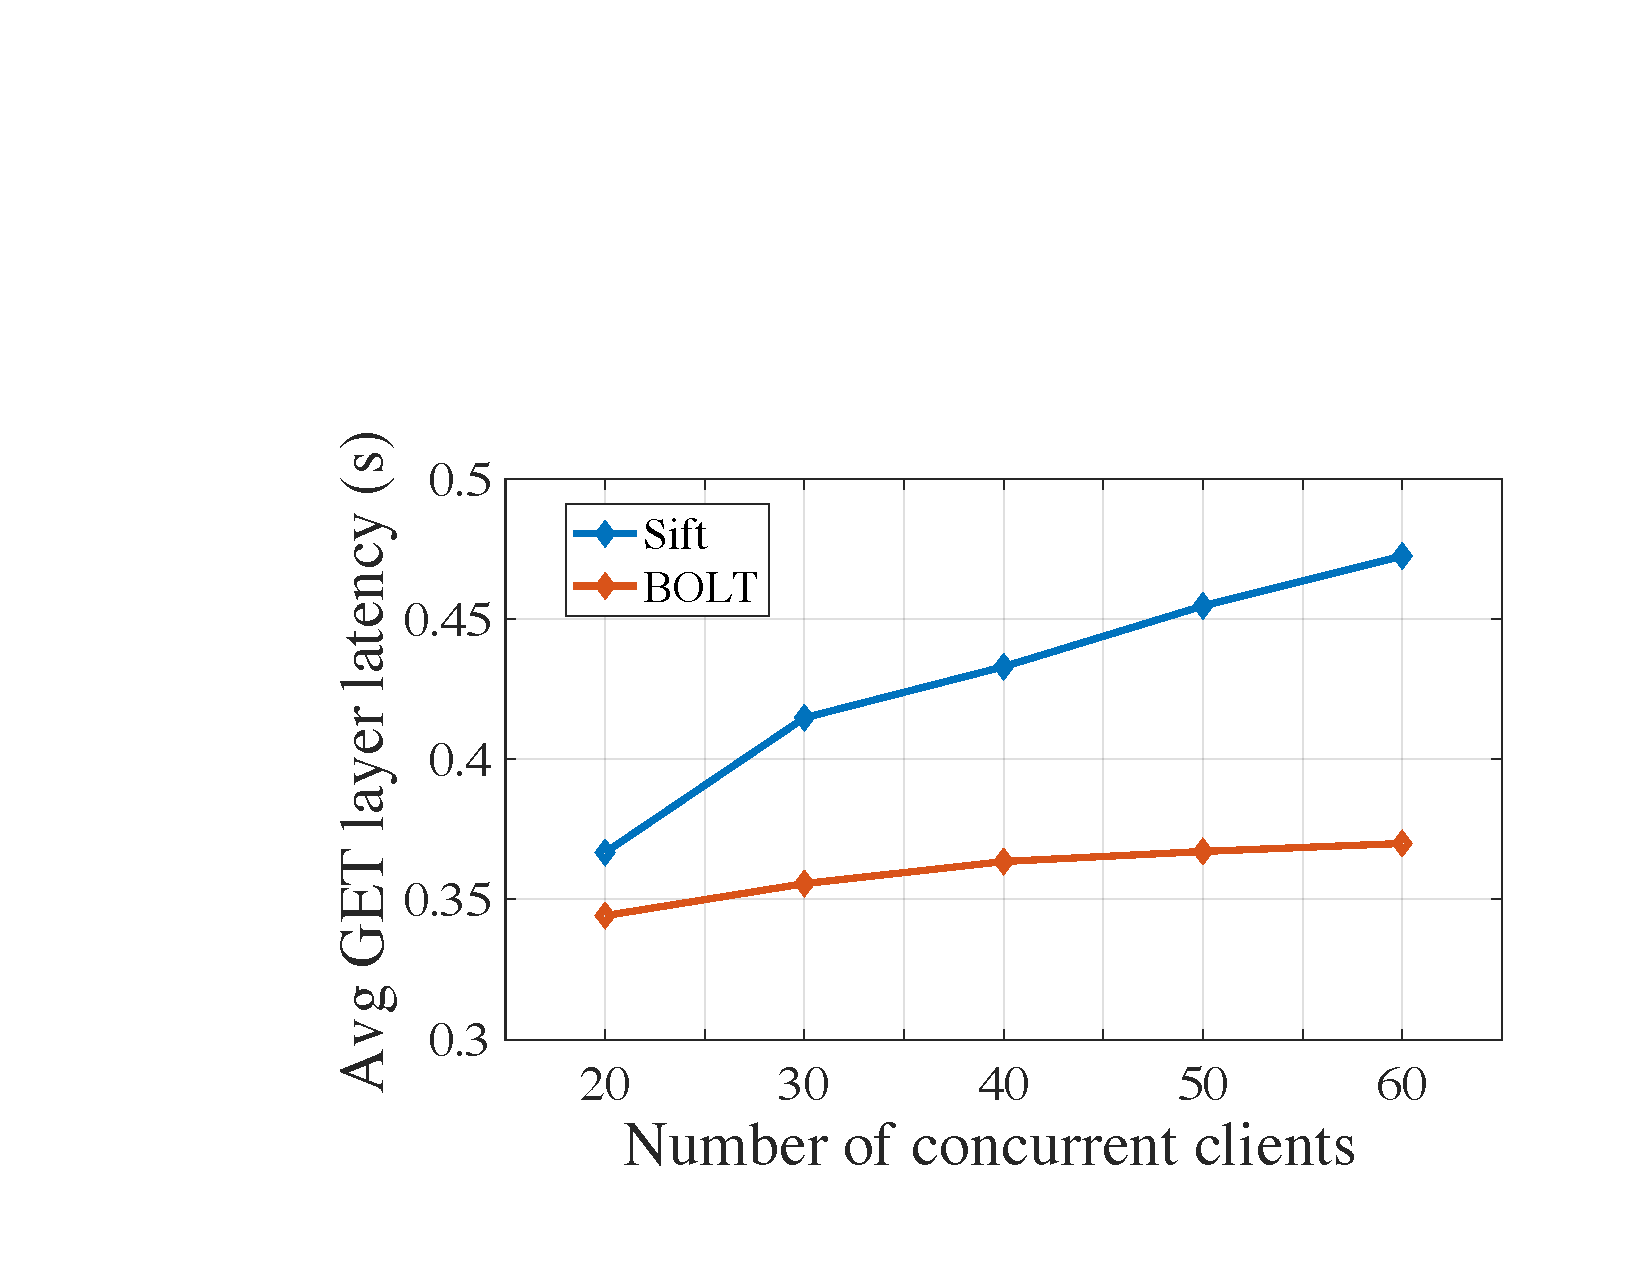
\includegraphics[width=\textwidth]{graphs/clientscale.pdf}
		\caption{GET layer latency with different client concurrency}
		\label{fig:eval-clientscale}
	\end{minipage}%
	\hspace{1mm}
	\begin{minipage}{0.3\textwidth}
	\centering
	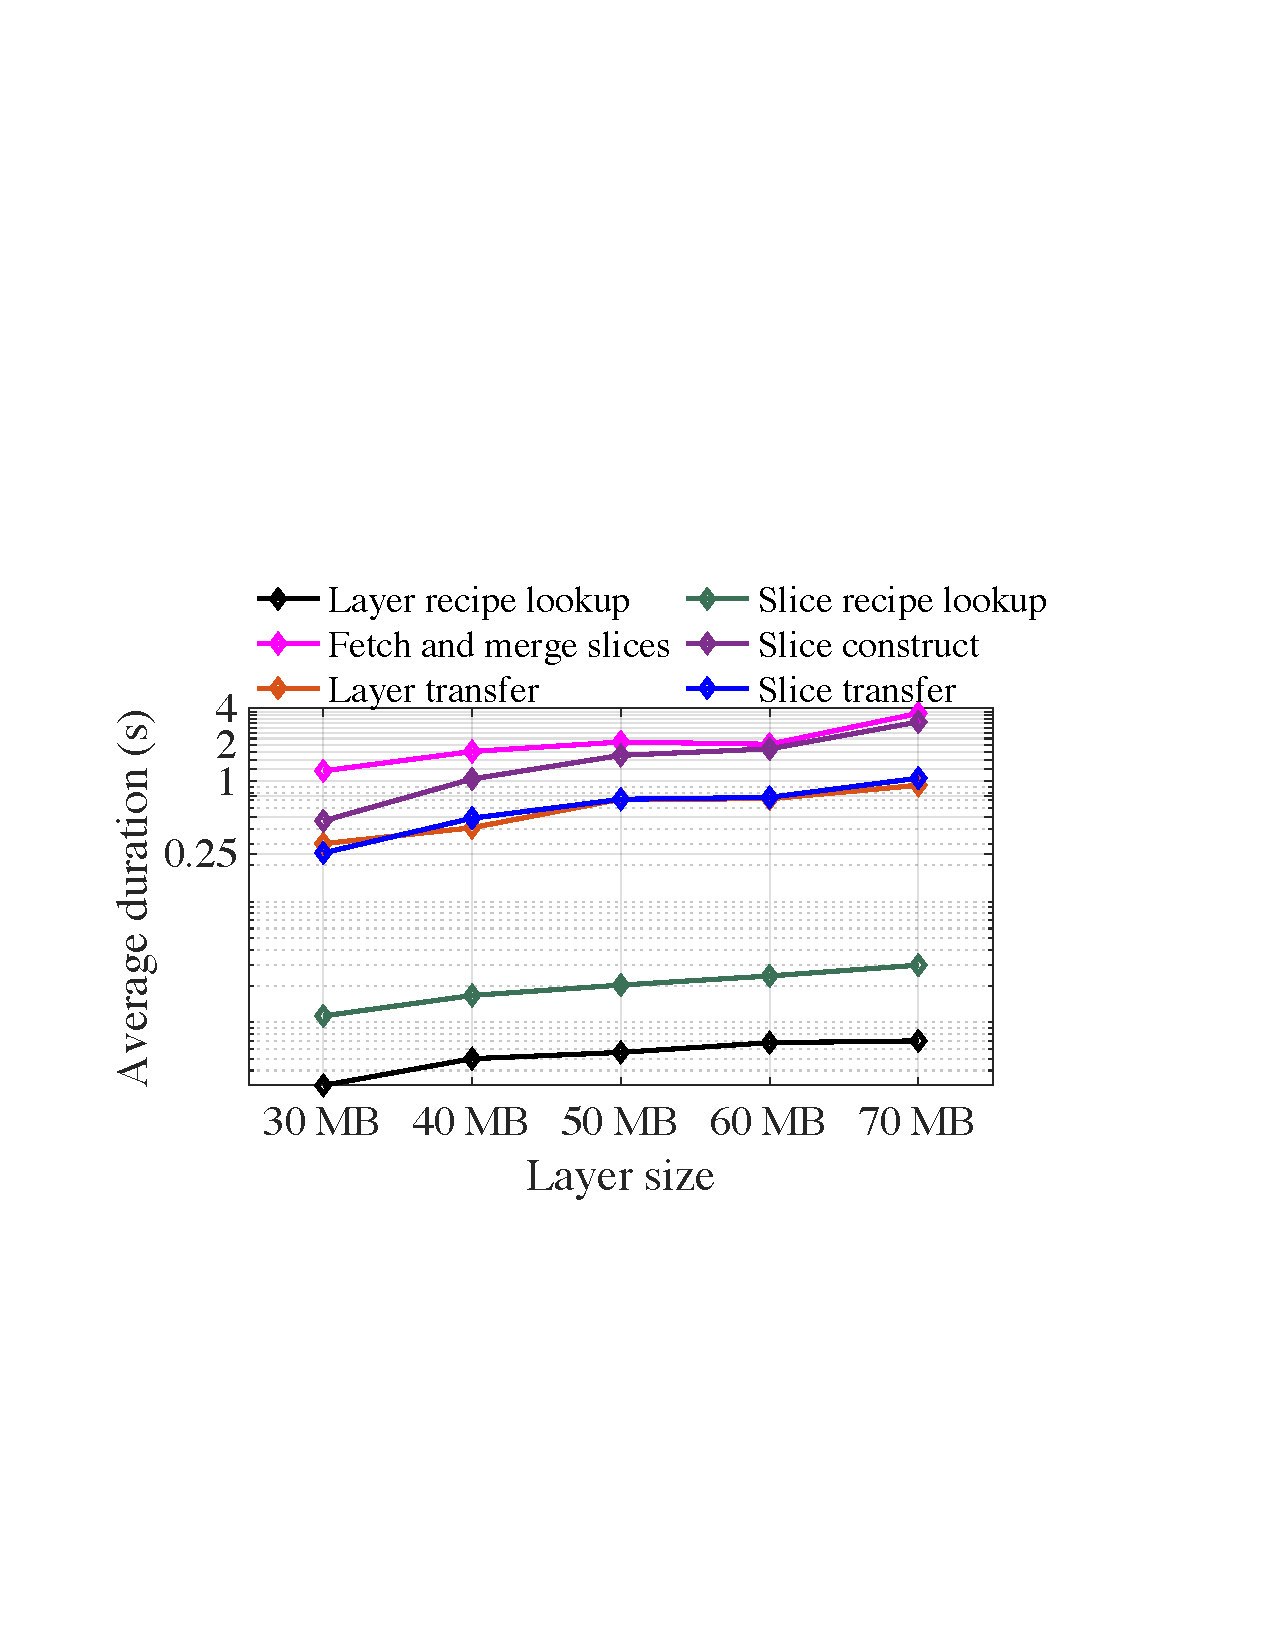
\includegraphics[width=\textwidth]{graphs/restoringbreakdown.pdf}
	\caption{Restoring latency breakdown}
	\label{fig:eval-restoringbreakdown}
	\end{minipage}
\end{figure*}

\begin{figure*}[t]
	\centering
	\begin{minipage}{0.3\textwidth}
		\centering
		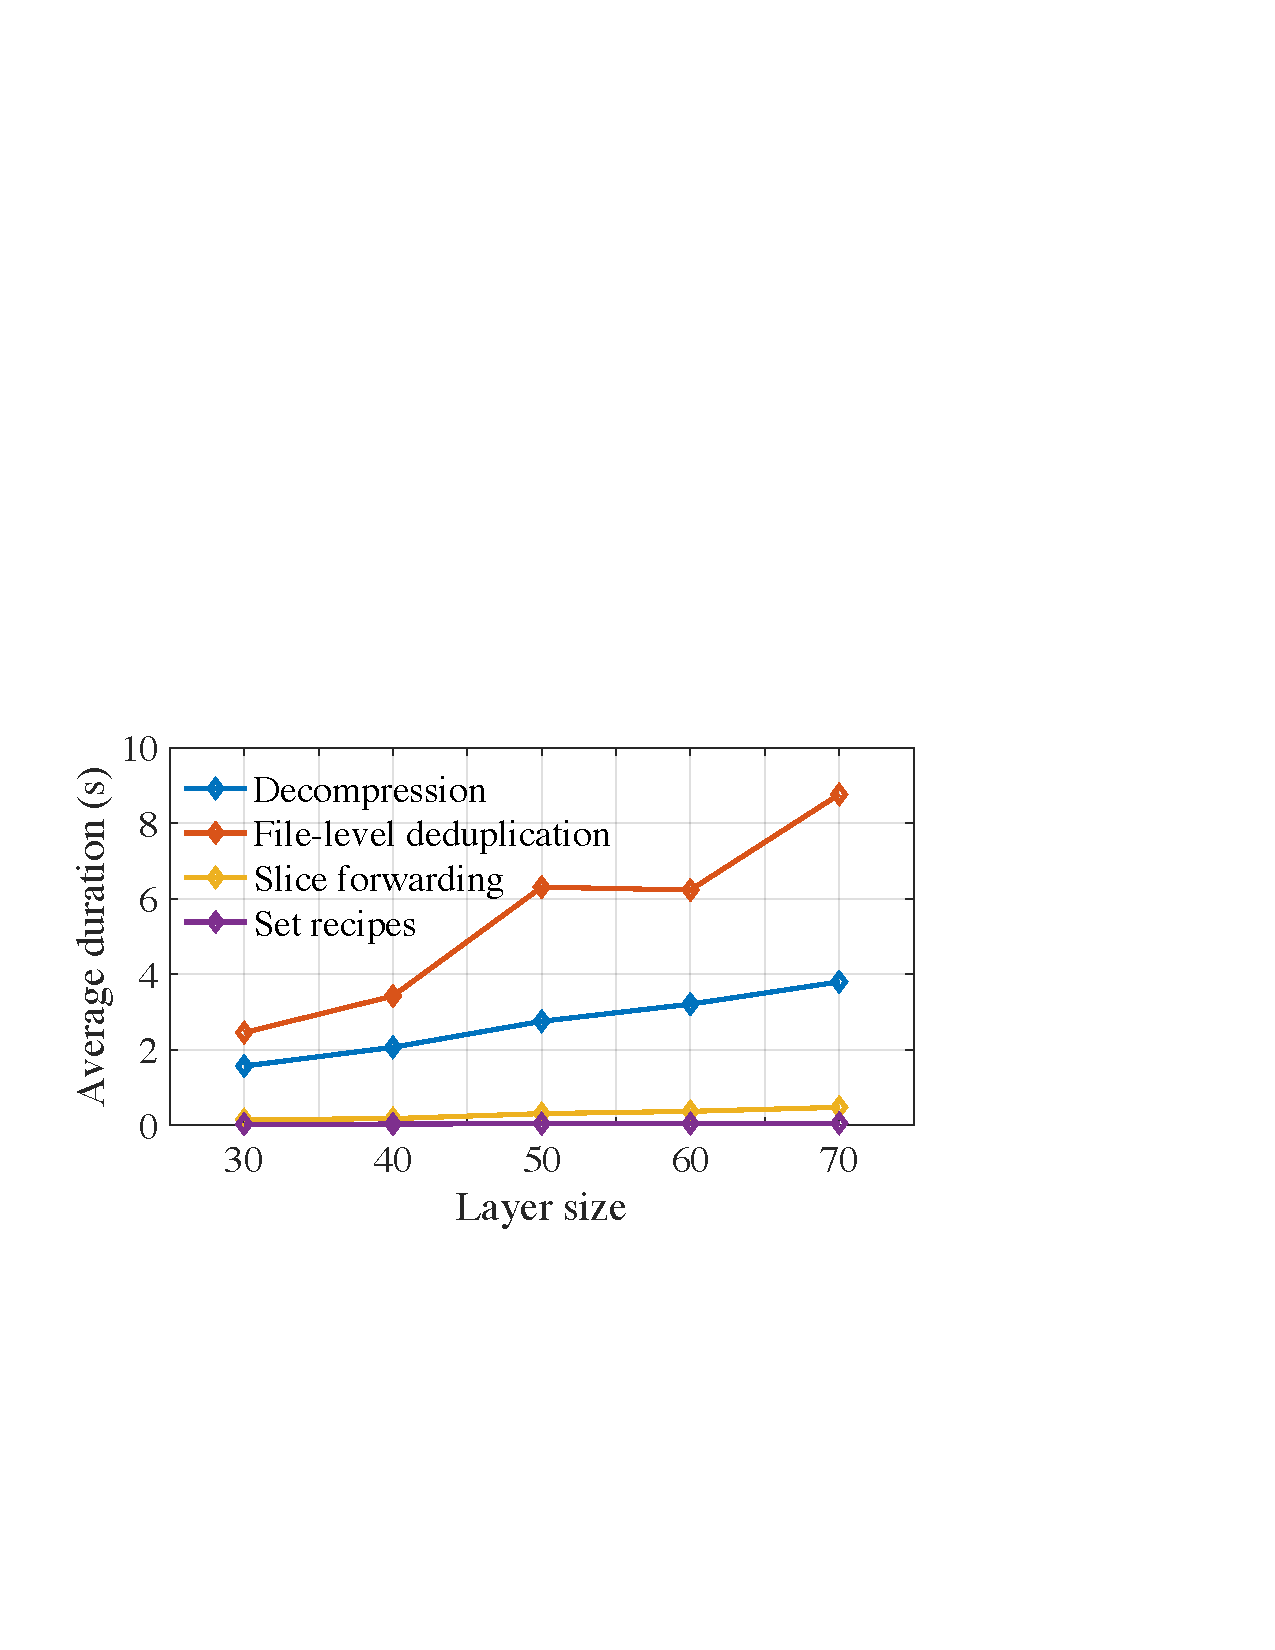
\includegraphics[width=\textwidth]{graphs/dedupbreakdown.pdf}
		\caption{Deduplication latency breakdown}
		\label{fig:eval-dedupbreakdown}
	\end{minipage}%
	\hspace{1mm}
	\begin{minipage}{0.3\textwidth}
		\centering
		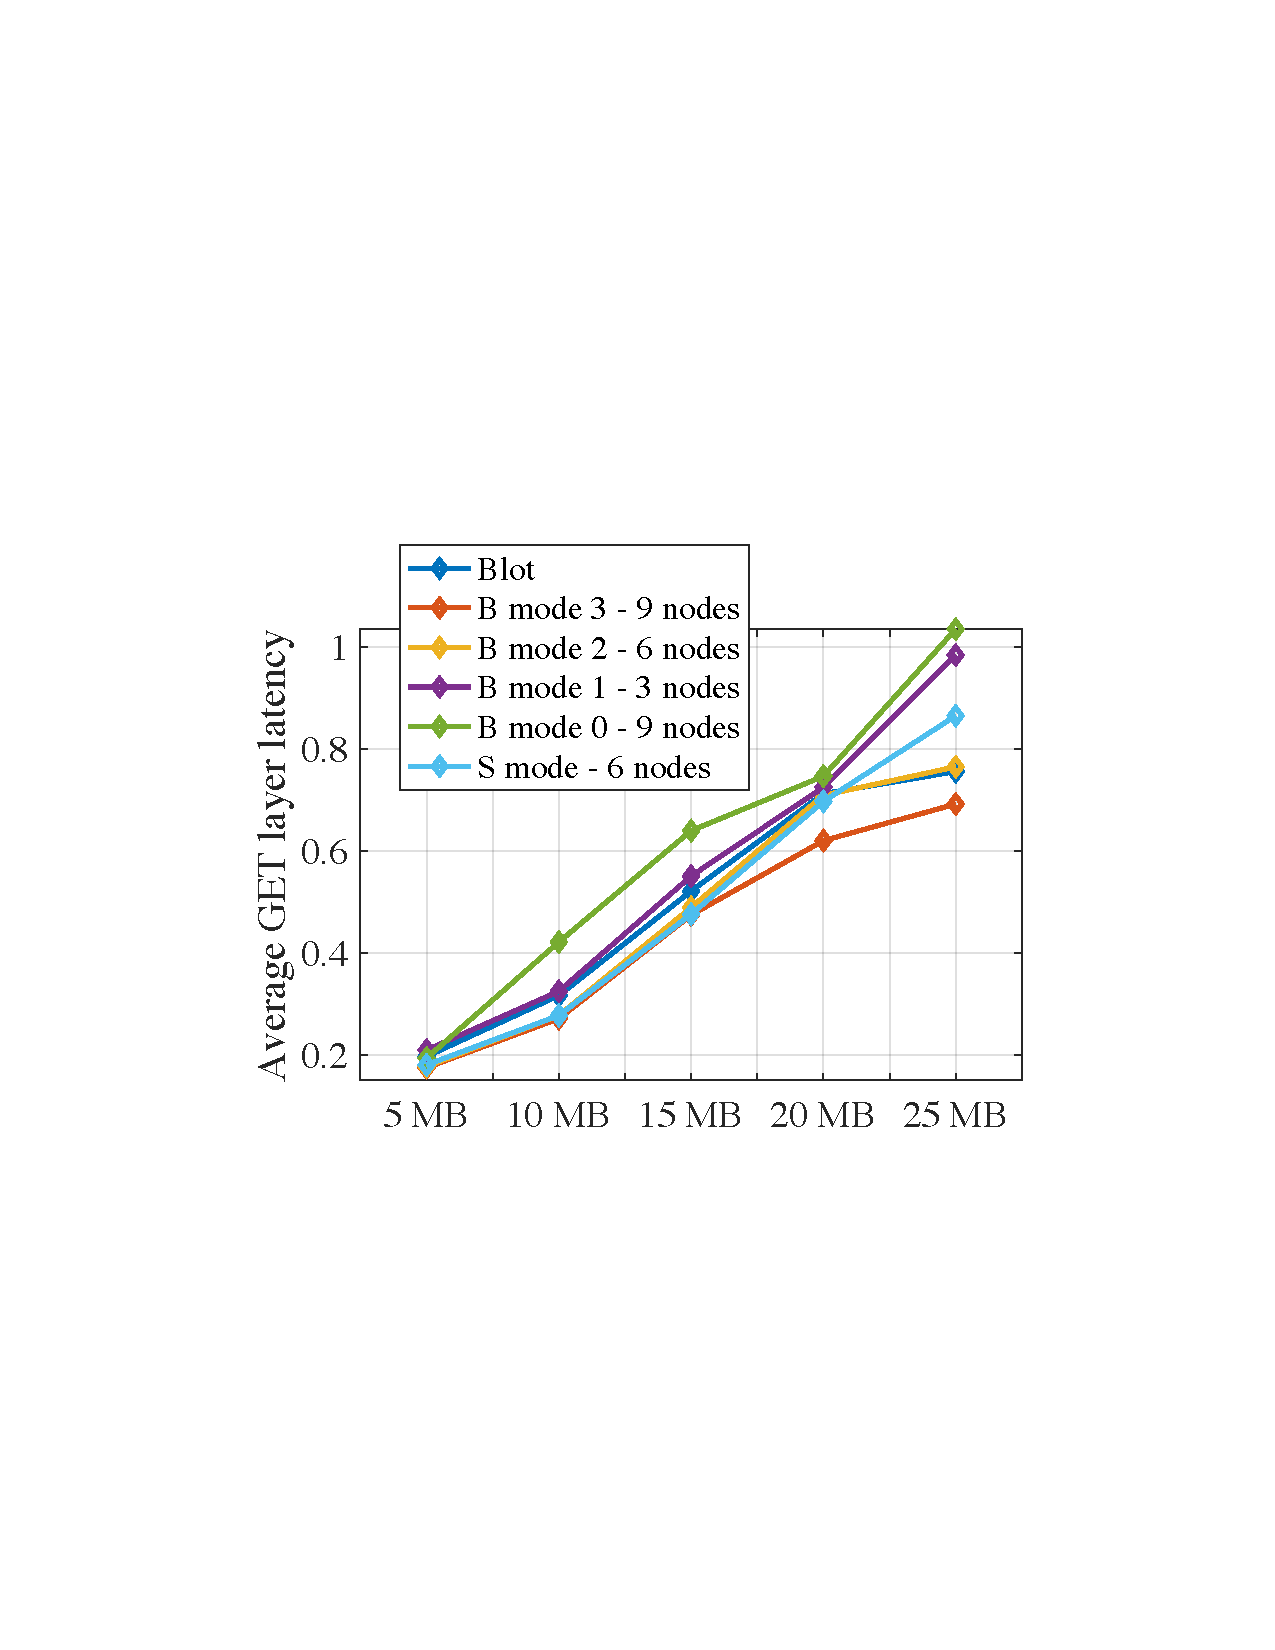
\includegraphics[width=\textwidth]{graphs/dalprimary.pdf}
		\caption{\texttt{GET} layer latency for different layer sizes}
		\label{fig:eval-dalprimary}
	\end{minipage}%
	\hspace{1mm}
	\begin{minipage}{0.3\textwidth}
		\centering
		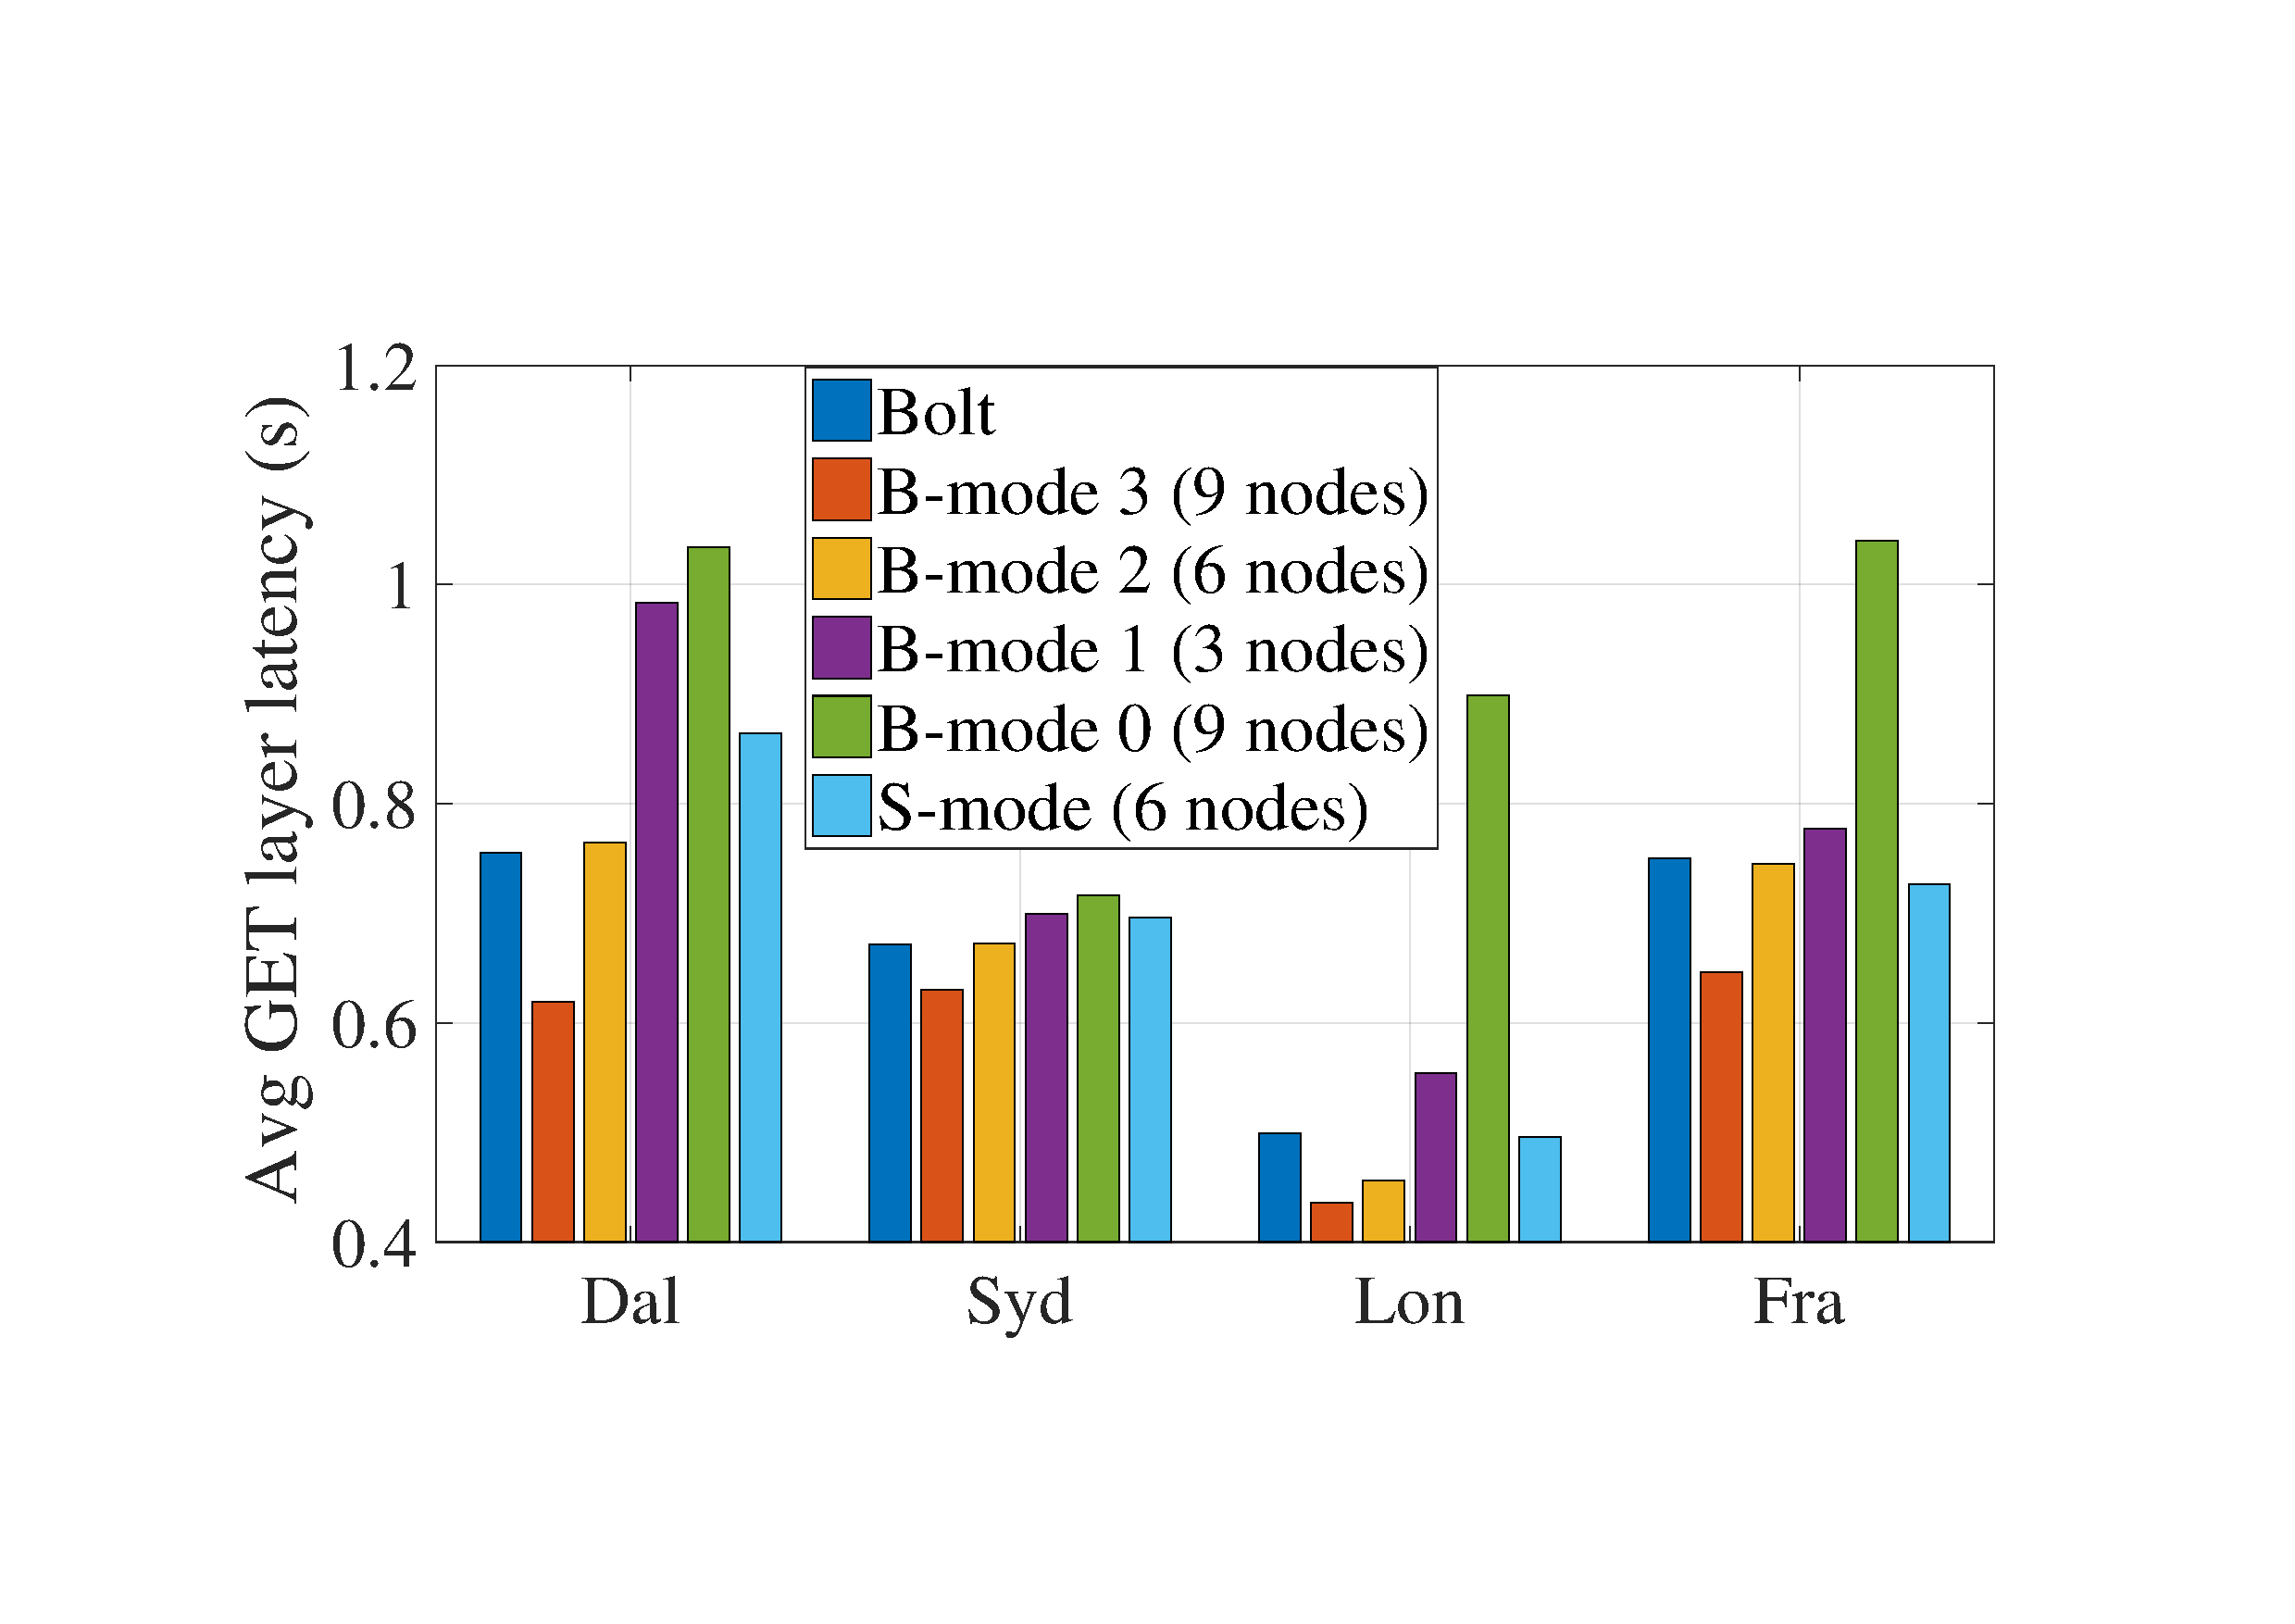
\includegraphics[width=\textwidth]{graphs/total-traces.pdf}
		\caption{\texttt{GET} layer latency for different workloads} %\Subil{"Blot" in figure should be "BOLT".}}
		\label{fig:eval-total-traces}
	\end{minipage}
\end{figure*}
 
\paragraph{Inter-arrival time of manifest and layer requests}
%
Next, we vary the inter-arrival time (IAT) between a \texttt{GET} manifest request and its
subsequent \texttt{GET} layer requests.
%
The layer size used here is 9~MB.
%
Figure~\ref{fig:eval-durationML} compares the average \texttt{GET} layer latency for
\sysname with preconstruct cache versus no deduplication.

When the IAT is 1\,s, \sysname with preconstruct cache only imposes a 19\% overhead.
%
However, as the IAT decreases, the average \texttt{GET} layer latency increases because
layers are not preconstructed in time.
%
When the client replays requests as fast as possible, the overhead of restoring layers on
\texttt{GET} layer requests increases by 30\%.
%
%\LR{How did we replay them in the previous experiment? As fast as possible or downsampled or in
%real-time?}
%\NZ{
%	First, there is an interval or delay between every two subsequent requests.
%	For \texttt{GET} manifest requests, we replay as fast as possible without delay.
%For \texttt{GET} layer requests,
%we use their real intervals if the intervals are smaller than 1 s. Otherwise,
%we use 1 s as the interval.
%We use the above method to replay traces for other tests (not for this different IAT test),
%This is for finishing all evaluations in a reasonable time.}

%the cache hit ratio of the ARC cache and the preconstruct cache.

\paragraph{Cluster scale out}
%
We analyze the impact of larger clusters and layers by increasing the number of registry servers from
7 to 14, and the layer sizes from 30 to 70\,MB and compare \sysname to the BOLT registry.
%
%(1) \sysname deduplication cluster (denoted as \sysname-dedup),
%and
%(2) BOLT \cite{littley2019bolt}.
Each registry server uses the local file system to store, and in the case of \sysname, deduplicate layers.
%
Similarly to BOLT, the consistent hashing logic is implemented at the client
side (see~\S\ref{sec:impl}) to route requests to the correct registry server.
 %Besides, 
 %that the client distributes layers to 
%Therefore,
%we also use our client to cluster the non-dededuplication registry servers and setup BOLT for evaluation.
We launch 20 clients on 2 servers to replay requests to the registries.

As shown in Figure~\ref{fig:eval-clusterscale}, BOLT achieves stable request latencies when
the number of registry servers increases.
%
While \sysname performs worse than BOLT, its performance improves with a larger cluster size.
%
This is because with a bigger deduplication cluster, layers can be restored faster due to higher
parallelism.
%
For example, for a layer size of 30\,MB, doubling the cluster size reduces the restoring
overhead by 35\%.

\paragraph{Workload scale up}
%
Next, we evaluate \sysname{}'s performance for an increasing workload.
%
We vary the number of concurrent client requests and measure the average \texttt{GET} layer
request latency on a 14-node cluster for \sysname and BOLT.
%
The results are shown in Figure~\ref{fig:eval-clientscale}.

BOLT only experiences a slight increase in \texttt{GET} layer latency as the number of clients increase.
%
On the other hand, latencies for \sysname increase linearly with the number of concurrent client requests.
%
For example, for 20 concurrent requests, the average \texttt{GET} layer latency is 0.37\,s which
increases to 0.47\,s for 60 concurrent requests.
%
This is because layer restoring is computationally intensive, i.e. for more concurrent requests, the CPU
becomes a bottleneck.

\paragraph{Restoring latency breakdown}
%
To analyze \sysname{}'s performance in more detail, we measure the time it takes
to reconstruct a layer and break the process down into its individual steps.
%
The steps in layer reconstruction include looking up the layer recipe, fetching and merging 
slices, and transferring the layer. Fetching and merging slices in itself involves slice recipe 
lookup, slice construction, and slice transfer.
%
%\LR{This is unclear, we've never talked about complete or waiting restoring processes before.
%What exactly are we doing here?}
%\NZ{We can delete "complete or waiting restoring processes" if it's confusing.
%"complete restoring processes" means the \texttt{GET} layer request misses on cache without
%layer preconstruction to wait.
%So this layer restoring process will have all the steps shown in  Figure~\ref{fig:eval-restoringbreakdown}.
%We count them in the figure.
%"waiting restoring processes" means the \texttt{GET} layer request misses cache but the request waits because
%layer preconstruction hasn't finished yet.
%So this layer restoring process will not have layer construct step. Instead it has a waiting step.
%We don't count them in the figure.
%Except for the above \texttt{GET} layer requests,
%we have \texttt{PRECONSTRUCT} layer requests.
%Those requests also initiate layer restoring processes, which contains all steps shown in
%Figure~\ref{fig:eval-restoringbreakdown}.
%We count them in the figure.}
%
%We only include complete layer restoring processes and eliminate the layer restoring processes
%that are waiting for others to construct layers.
%
%\LR{Again, the following is confusing. What does it mean?}
%\NZ{we count the layer restoring processes for both \texttt{GET} layer requests and
%\texttt{PRECONSTRUCT} layer requests.}
%
%Note that the layer restoring latencies measured also include layer restoring processes for preconstruction.
%
The latencies are measured on the 7-node cluster and the breakdown is shown in
Figure~\ref{fig:eval-restoringbreakdown}.

We can see that slice reconstruction accounts for the largest portion of layer construction time.
%
Slice construction involves file archiving and compression, which are the main bottlenecks.
%. 
Layer construction time increases with layer size because layer slices become bigger and
take longer to archive and compress.
%
For example, for layers of size 30\,MB, fetching and merging slices takes 1.3\,s on average while
for 70\,MB layers, it takes 3.6\,s.

\paragraph{Deduplication latency breakdown}
%
Finally, we study the deduplication process in more detail.
%
Note that to reduce the impact of layer deduplication on the \texttt{GET} layer request,
the layer deduplication process runs in off-line mode.
%
Figure~\ref{fig:eval-dedupbreakdown} shows the breakdown of the deduplication latency.

We observe that decompression and file-level deduplication account for the largest portions of
the layer deduplication duration.
%
%\LR{Why does the following reduce the overhead? Do we want to reduce the impact on the
%restoring processes?}
%\NZ{Because there are \texttt{GET} and \texttt{PUT} requests.
%We configure deduplication process to use a single thread to 
%minimize its computation and I/O resource consumption
%so it wont compete for resources with layer restoring process. }
%
This is because \sysname uses single-threaded decompression and file-level deduplication in
order to reduce interference with the critical layer restoration processes.
%
%\Subil{This conflicts with our description of pgzip in the Implementation section where we
% talk about using parallelism in both compression ad decompression}.
%\NZ{pgzip is for layer restoring. We use standard gzip for deduplication.}
%\Subil{Since we are only using pgzip for compression for layer restoring for pulls and standard
%gzip for decompression during a push, we should remove the implication that pgzip is used
%for both compression and decompression at the end of section 5.2}
%
Moreover, the duration of decompression and file-level deduplication increases with layer sizes.
%
For example, when the layer size increases from 30\,MB to 70\,MB, 
the decompression duration increases from 1.6\,s to 3.8\,s on average and the file-level deduplication duration increases from 2.5\,s to 8.8\,s on average.
%
This is expected as more data needs to be processed.
%\paragraph{Metadata size} 
%Figure~\ref{xxx} shows the average metadata size on each registry server measured by using the size of the used memory in Redis~\cite{redis} when in \emph{B-mode 0}.
%Note that the replication level for the Redis cluster is also set to three.
%As shown, for all traces, the total size of the metadata generated by \sysname such as \emph{recipes} for layers or slices, \emph{indexes} of layers or files, and RLmap or ULmap is less than 100 MB.
%With the 16 GB memory on each registry server, such metadata size is negligible.


